\documentclass[letter,12pt]{article}
\usepackage[letterpaper,right=1in,left=1in,top=1in,bottom=1in]{geometry}
\usepackage{setspace}

\usepackage[utf8]{inputenc}   % allows input of special characters from keyboard (input encoding)
\usepackage[T1]{fontenc}      % what fonts to use when printing characters       (output encoding)
\usepackage{amsmath}          % facilitates writing math formulas and improves the typographical quality of their output
\usepackage[hyphens]{url}     % adds line breaks to long urls
\usepackage[pdftex]{graphicx} % enhanced support for graphics
\usepackage{tikz}             % Easier syntax to draw pgf files (invokes pgf automatically)
\usetikzlibrary{arrows}

\usepackage{mathptmx}           % set font type to Times
\usepackage[scaled=.90]{helvet} % set font type to Times (Helvetica for some special characters)
\usepackage{courier}            % set font type to Times (Courier for other special characters)

\usepackage[longnamesfirst, sort]{natbib}\bibpunct[]{(}{)}{,}{a}{}{;} % handles biblio and references 

\usepackage{rotating}         % sideway tables and figures that take a full page
\usepackage{caption}          % allows multipage figures and tables with same caption (\ContinuedFloat)

\usepackage{dcolumn}          % needed for apsrtable and stargazer tables from R to compile
\usepackage{arydshln}         % dashed lines in tables (hdashline, cdashline{3-4}, 
                              %see http://tex.stackexchange.com/questions/20140/can-a-table-include-a-horizontal-dashed-line)
                              % must be loaded AFTER dcolumn, 
                              %see http://tex.stackexchange.com/questions/12672/which-tabular-packages-do-which-tasks-and-which-packages-conflict


\newcommand{\mc}{\multicolumn}

\usepackage{epigraph}          % format epigraphs

%% TO ADD NOTES IN TEXT, PUT % BEFORE THE ONE YOU WANT DISABLED
%\usepackage[disable]{todonotes}                            % no show
\usepackage[colorinlistoftodos, textsize=small]{todonotes} % show notes
\newcommand{\emm}[1]{\todo[color=red!15, inline]{\textbf{Eric:} #1}}

%% \usepackage{xr} % allows cross-ref to other file
%% \externaldocument{urge15appendix}

%% %for submission: sends figs, tables, and footnotes to last pages
%% \RequirePackage[nomarkers,nolists]{endfloat}     % sends tables and figures to the end
%% \RequirePackage{endnotes}                        % turns fn into endnotes; place \listofendnotes where you want 
%%                                                  %the endnotes to appear (it must be after the last endnote).
%% \let\footnote=\endnote
%% \newcommand{\listofendnotes}{
%%    \begingroup
%%    \parindent 0pt
%%    \parskip 2ex
%%    \def\enotesize{\normalsize}
%%    \theendnotes
%%    \endgroup
%% }
%% 
%% % for submission: drop page numbers when producing title page
%% \pagenumbering{gobble} % Remove page numbers (and reset to 1)
%% \pagenumbering{arabic}% Arabic page numbers (and reset to 1)


\setcitestyle{citesep={;}}

\usepackage{listings}

\begin{document}

\title{Appendix to Floor access in Mexico's Cámara de Diputados\thanks{Eric Magar received financial support from the Asociaci\'on Mexicana de Cultura \textsc{a.c.}\ and \textsc{conacyt}'s Sistema Nacional de Investigadores. For shedding light on major parties' internal rules of debate in the period, I thank Fernando Rodríguez Doval, Lupita Vargas Vargas, and one former lawmaker who wished anonymity. I am grateful to Ana Lucía Enríquez Araiza, Sonia Kuri Kosegarten, Vidal Mendoza Tinoco, and Eugenio Solís Flores, for research assistance. The author is responsible for mistakes and shortcomings in the study. Data and supporting materials necessary to reproduce the quantitative analysis are available at \url{https://github.com/emagar/legdeb}.}}
\author{Eric Magar \\ Instituto Tecnológico Autónomo de México}
\date{\today}
\maketitle

\newpage

\doublespacing

\section{Appendix}

\subsection{Party shares in the Cámara}

\begin{table}
\begin{scriptsize}
\begin{verbatim}
|----------------------------+---------+---------+---------|
|                            |    60th |    62nd |    64th |
|                            | 2006-09 | 2012-15 | 2018-21 |
| Party                      |       % |       % |       % |
|----------------------------+---------+---------+---------|
| pan                        |      41 |      23 |      16 |
| pri                        |      21 |      43 |       9 |
| prd                        |      25 |      20 |       4 |
| morena                     |         |         |      51 |
| opportunistic w/ president |         |       8 |      14 |
| other opportunistic        |      13 |       7 |       6 |
|----------------------------+---------+---------+---------|
| Total                    % |     100 |     100 |     100 |
| N                          |     500 |     500 |     500 |
|----------------------------+---------+---------+---------|
| President's party          |     pan |     pri |  morena |
|----------------------------+---------+---------+---------|
\end{verbatim}
\end{scriptsize}
\caption{Parties in three Legislatures of the Cámara de Diputados}\label{T:seats}
\end{table}

%% |              |  60 |  62 |     64 |
%% |              |   N |   N |      N |
%% |--------------+-----+-----+--------+
%% | pan          | 207 | 114 |     79 |
%% | pri          | 104 | 213 |     47 |
%% | prd          | 125 | 102 |     20 |
%% | morena       |     |     |    255 |
%% | opport w pdt |     |  38 |     69 |
%% | oth opport   |  64 |  33 |     30 |
%% |--------------+-----+-----+--------+
%% | Total        | 500 | 500 |    500 |


\subsection{Women representation and debate}

\begin{table}
  \begin{scriptsize}
    \begin{verbatim}
|                   | % women |    of |
|-------------------+---------+-------|
| Members           |      39 |  1710^|
| -60th             |      28 |   603 |
| -62nd             |      41 |   640 |
| -64th             |      47 |   531 |
| Cámara presidents |      35 |    31 |
| Committee chairs  |      28 |   174 |
| Party leaders     |      21 |    24 |
| - major party     |       0 |    12 |
| - opportunistic   |      42 |    12 |
| Speechmakers      |      37 |  5926 |
| Speeches          |      41 | 23637 |
| Words spoken      |      41 | 17.5M |
|-------------------+---------+-------|
|^Returning members counted once only.|
|-------------------+---------+-------|
    \end{verbatim}
  \end{scriptsize}
\caption{Women representation and debate}\label{T:women}
\end{table}



\subsection{Dependent variable summary statistics}

Figure \ref{F:dv-hist} describes both flavors of the dependent variables. And Figure \ref{F:quantiles} portrays member daily aggregates across the periods analyzed. For clarity, this plot includes speakers only (keep in mind that non-speakers are included in the period aggregates analyzed.)

\begin{figure}
  \centering
  \begin{tabular}{cc}
    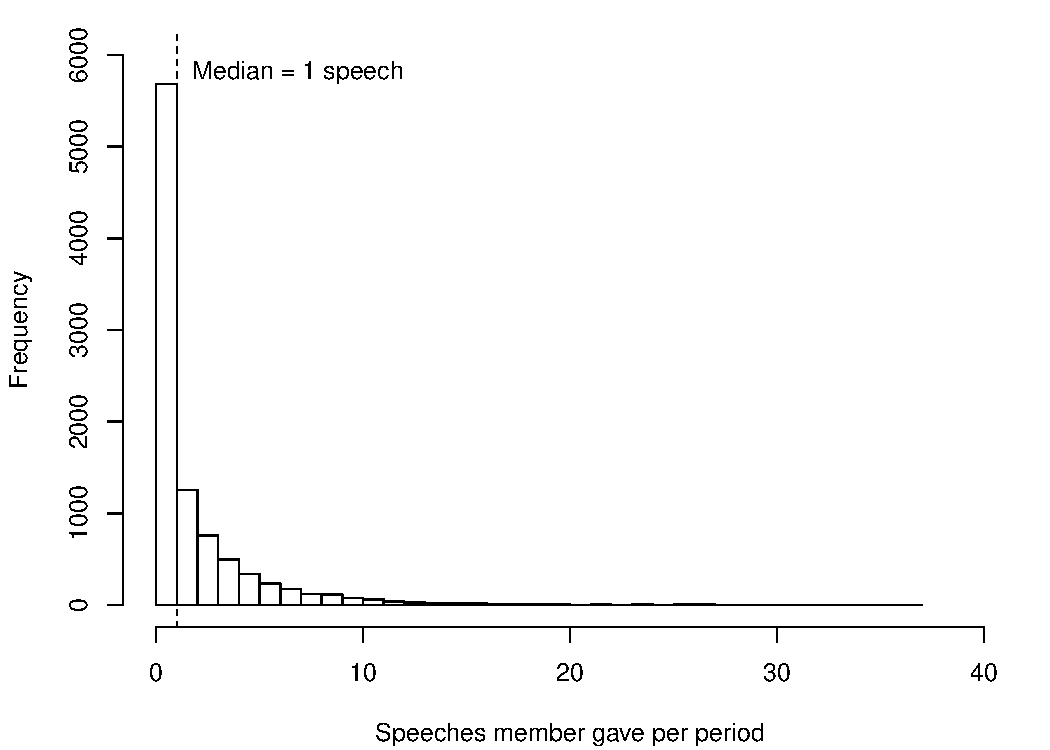
\includegraphics[width=.49\columnwidth]{../plots/dv-nspeech-histogram.pdf} &
    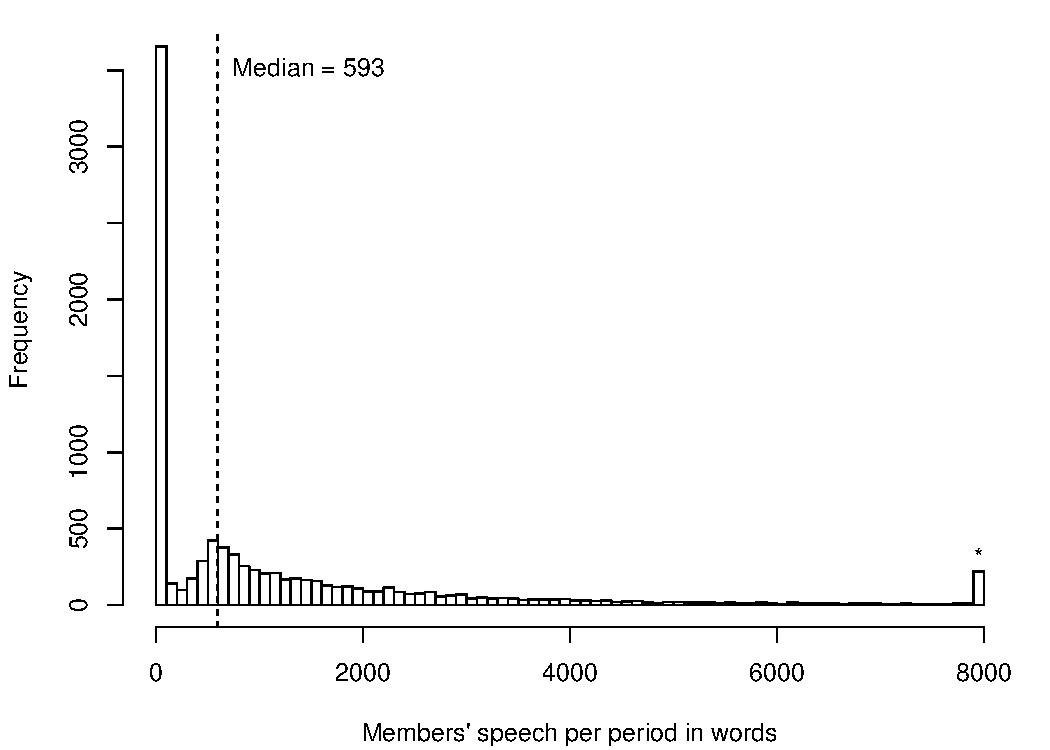
\includegraphics[width=.49\columnwidth]{../plots/dv-histogram.pdf}
  \end{tabular}
    \caption{The dependent variable, number of speeches (left) and number of words (right). The column under a star in the right panel is cumulative, reporting 217 member-periods with 8 thousand words or more (2.2 percent of all, the actual distribution spreads these observations, with increasing sparseness, from 8000 to 50291).}\label{F:dv-hist}
\end{figure}


%% \begin{figure}
%%   \centering
%%     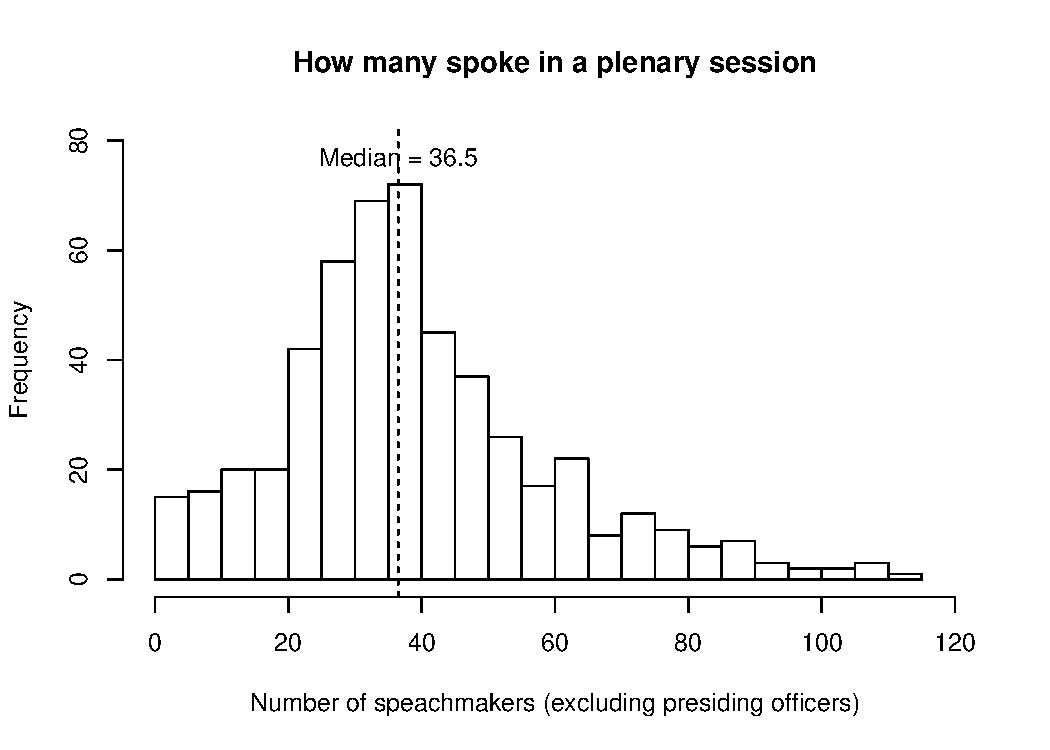
\includegraphics[width=.8\columnwidth]{../plots/nspeakers.pdf}
%%     \caption{Number of daily speakers}\label{F:nspeakers}
%% \end{figure}


\begin{figure}
  \centering
    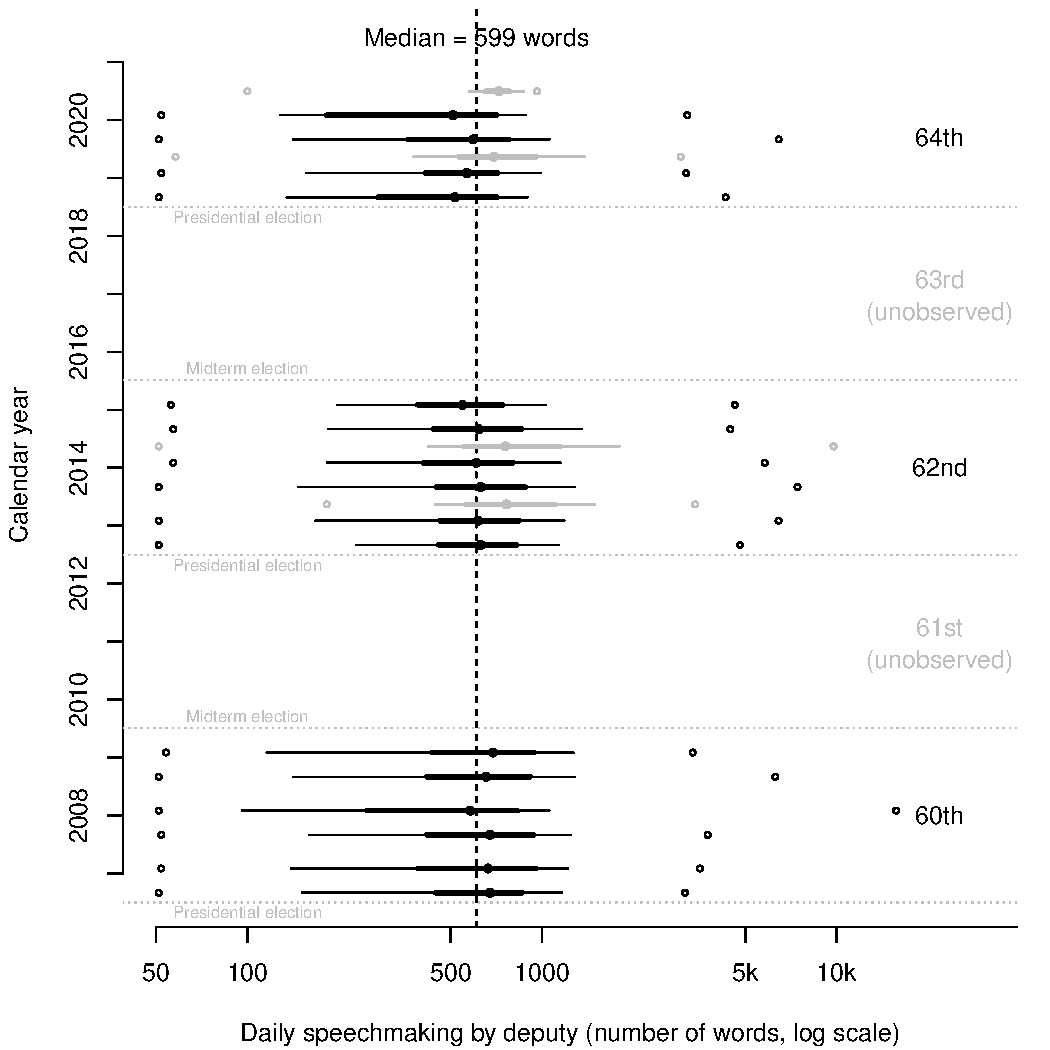
\includegraphics[width=.5\columnwidth]{../plots/quantiles-periodo.pdf}
    \caption{Daily speech length by legislative period observed. The plot excludes non-speaking members. Solid points indicate the median speech length in the period. Thick and thin lines connect the 25--75 and 10--90 percentiles, respectively. Hollow points are minima and maxima. Ordinary periods in black, extraordinary periods in gray.}\label{F:quantiles}
\end{figure}

%The log scale magnifies the low side of the distribution. But it also blurs subtle but revealing differences in the high side. From 60th to 62nd, max went up while percentiles 75 and 90 remain at similar levels. Like Batres, an unusually high top decile consists of attempts to disrupt debate through filibustering. Dilatory tactics went down in 62nd compared with 60th, and substantially so in the 64th with a single party majority.


%% \singlespacing
%% \begin{footnotesize}
%% \begin{verbatim}
%% Words per day
%% | Legislatura    | min | 10% | 25% | 50% | 75% |  90% |   max |
%% | 60th           |  50 | 137 | 392 | 652 | 901 | 1215 | 15932 |
%% | 62nd           |  50 | 193 | 438 | 611 | 850 | 1254 |  9765 |
%% | 64th (partial) |  50 | 142 | 327 | 547 | 730 |  975 |  6358 |
%% \end{verbatim}
%% \end{footnotesize}
%% \doublespacing



%% \subsection{Alternative model specifications}

%% Forthcoming. 

%% \begin{table} \centering 
%%   \begin{tiny}
%%     \begin{verbatim}
%% ==================================================================================================================================
%%                                     DV = Words/exposure in period                                  DV = Words in period               
%%                       --------------------------------------------------------------   -------------------------------------------
%%                               (1)                       (2)                 (3)            (4)             (5)            (6)     
%% ----------------------------------------------------------------------------------------------------------------------------------
%% Exposure (logged)                                                                        0.93***         0.95***        0.34***   
%%                                                                                          (0.04)          (0.04)         (0.02)    
                                                                                                                                  
%% Majority                  1,029.48***               1,489.83***          835.24***       1.03***         1.04***        0.78***   
%%                             (91.07)                  (137.37)            (226.39)        (0.09)          (0.14)         (0.06)    
                                                                                                                                  
%% Party leader              2,186.15***               1,972.75***         1,309.31***       0.40*           0.33          0.28***   
%%                             (206.55)                 (205.36)            (310.46)        (0.21)          (0.21)         (0.07)    
                                                                                                                                  
%% Comm. chair                247.65***                  139.20               88.01         0.37***         0.32***        0.14***   
%%                             (89.79)                   (89.29)            (152.24)        (0.09)          (0.09)         (0.04)    
                                                                                                                                  
%% Seniority                  145.30***                 180.04***           203.98**        0.16***         0.17***        0.12***   
%%                             (48.19)                   (47.59)             (85.93)        (0.05)          (0.05)         (0.02)    
                                                                                                                                  
%% Woman                      164.02***                 125.84**              17.03          0.08            0.07           0.03     
%%                             (54.92)                   (54.94)             (99.85)        (0.06)          (0.06)         (0.02)    
                                                                                                                                  
%% Party size                 -67.81***                 -72.36***           -63.36***      -0.05***        -0.05***       -0.04***   
%%                              (2.00)                   (2.26)              (3.85)         (0.002)         (0.002)        (0.001)   
                                                                                                                                  
%% SMD                          -38.64                   -106.08             -121.47         -0.03           -0.10          -0.03    
%%                             (55.93)                   (65.04)            (115.72)        (0.06)          (0.07)         (0.03)    
                                                                                                                                  
%% SMD x reelect                                        267.50**              3.43                          0.26**         0.11**    
%%                                                      (120.97)            (189.85)                        (0.12)         (0.05)    
                                                                                                                                  
%% Suplente                   -310.36***               -379.09***           -354.13**      -0.35***        -0.36***       -0.35***   
%%                             (110.62)                 (109.03)            (140.76)        (0.11)          (0.11)         (0.05)    
                                                                                                                                  
%% 62nd Leg.                                            689.82***           825.22***                       0.18***        0.08***   
%%                                                       (63.01)             (96.98)                        (0.06)         (0.03)    
                                                                                                                                  
%% 64th Leg.                                             -118.71            523.90***                        -0.09        -0.21***   
%%                                                      (114.65)            (165.78)                        (0.12)         (0.04)    
                                                                                                                                  
%% Extraordinary                                      -1,101.73***        -1,109.15***                                               
%%                                                       (73.24)             (48.29)                                                 
                                                                                                                                  
%% Constant                  3,119.59***               3,122.09***         2,829.41***      5.22***         5.09***        7.26***   
%%                             (70.98)                   (86.15)            (144.04)        (0.14)          (0.16)         (0.08)    
                                                                                                                                  
%% ----------------------------------------------------------------------------------------------------------------------------------
%% Fixed effects                  no                      term                term            no             term           term
%% Random effects                 no                       no                member           no              no             no
%% Estimation method             OLS                      OLS                linear         negative        negative    zero-inflated
%%                                                                        mixed-effects     binomial        binomial     count data   
%% ----------------------------------------------------------------------------------------------------------------------------------
%% Observations                 9,494                     9,494               9,494          9,494           9,494          9,494    
%% R2                            0.15                     0.18                                                                       
%% Adjusted R2                   0.15                     0.17                                                                       
%% Log Likelihood                                                          -85,190.54     -60,825.36      -60,818.74     -55,503.49  
%% theta                                                                                0.16*** (0.002) 0.16*** (0.002)              
%% Akaike Inf. Crit.                                                       170,411.10     121,670.70      121,663.50                 
%% Bayesian Inf. Crit.                                                     170,518.50                                                
%% Residual Std. Error   2,506.13 (df = 9485)     2,467.49 (df = 9481)                                                               
%% F Statistic         208.32*** (df = 8; 9485) 168.54*** (df = 12; 9481)
%% LR test intercept-only      
%% ==================================================================================================================================
%% Note:                                                                                                  *p<0.1; **p<0.05; ***p<0.01
%% \end{verbatim}
%%   \end{tiny}
%%   \caption{Models of legislative debate. Standard errors in parentheses. } 
%%   \label{T:app-regs} 
%% \end{table} 

%\listofendnotes

\newpage

\singlespacing

\bibliographystyle{apsr}

\bibliography{../bib/magar}

%% \begin{thebibliography}{xx}

%% \harvarditem{Alem\'an \harvardand\ Tsebelis}{2016}{aleman-tsebelis-2016-book}
%% Alem\'an, Eduardo \harvardand\ George Tsebelis. 2016.
%% \newblock {\em Legislative Institutions and Lawmaking in Latin America}.
%% \newblock Oxford:  Oxford University Press.

%% \harvarditem{Alem\'an \harvardand\ Navia}{2009}{aleman.navia.UrgChi.2009}
%% Alem\'an, Eduardo \harvardand\ Patricio Navia. 2009.
%% \newblock ``Institutions and the Legislative Success of `Strong' Presidents: An
%%   Analysis of Government Bills in {Chile}.'' {\em Journal of Legislative
%%   Studies} 15(4):401--19.

%% \end{thebibliography}


\end{document}

